\chapter{SOLID}

\section{Analyse Single-Responsibility-Principle (SRP)}
[jeweils eine Klasse als positives und negatives Beispiel für SRP;  jeweils UML der Klasse und Beschreibung der Aufgabe bzw. der Aufgaben und möglicher Lösungsweg des Negativ-Beispiels (inkl. UML)]
\subsection{Positiv-Beispiel}
\begin{figure}[H]
	\centering
	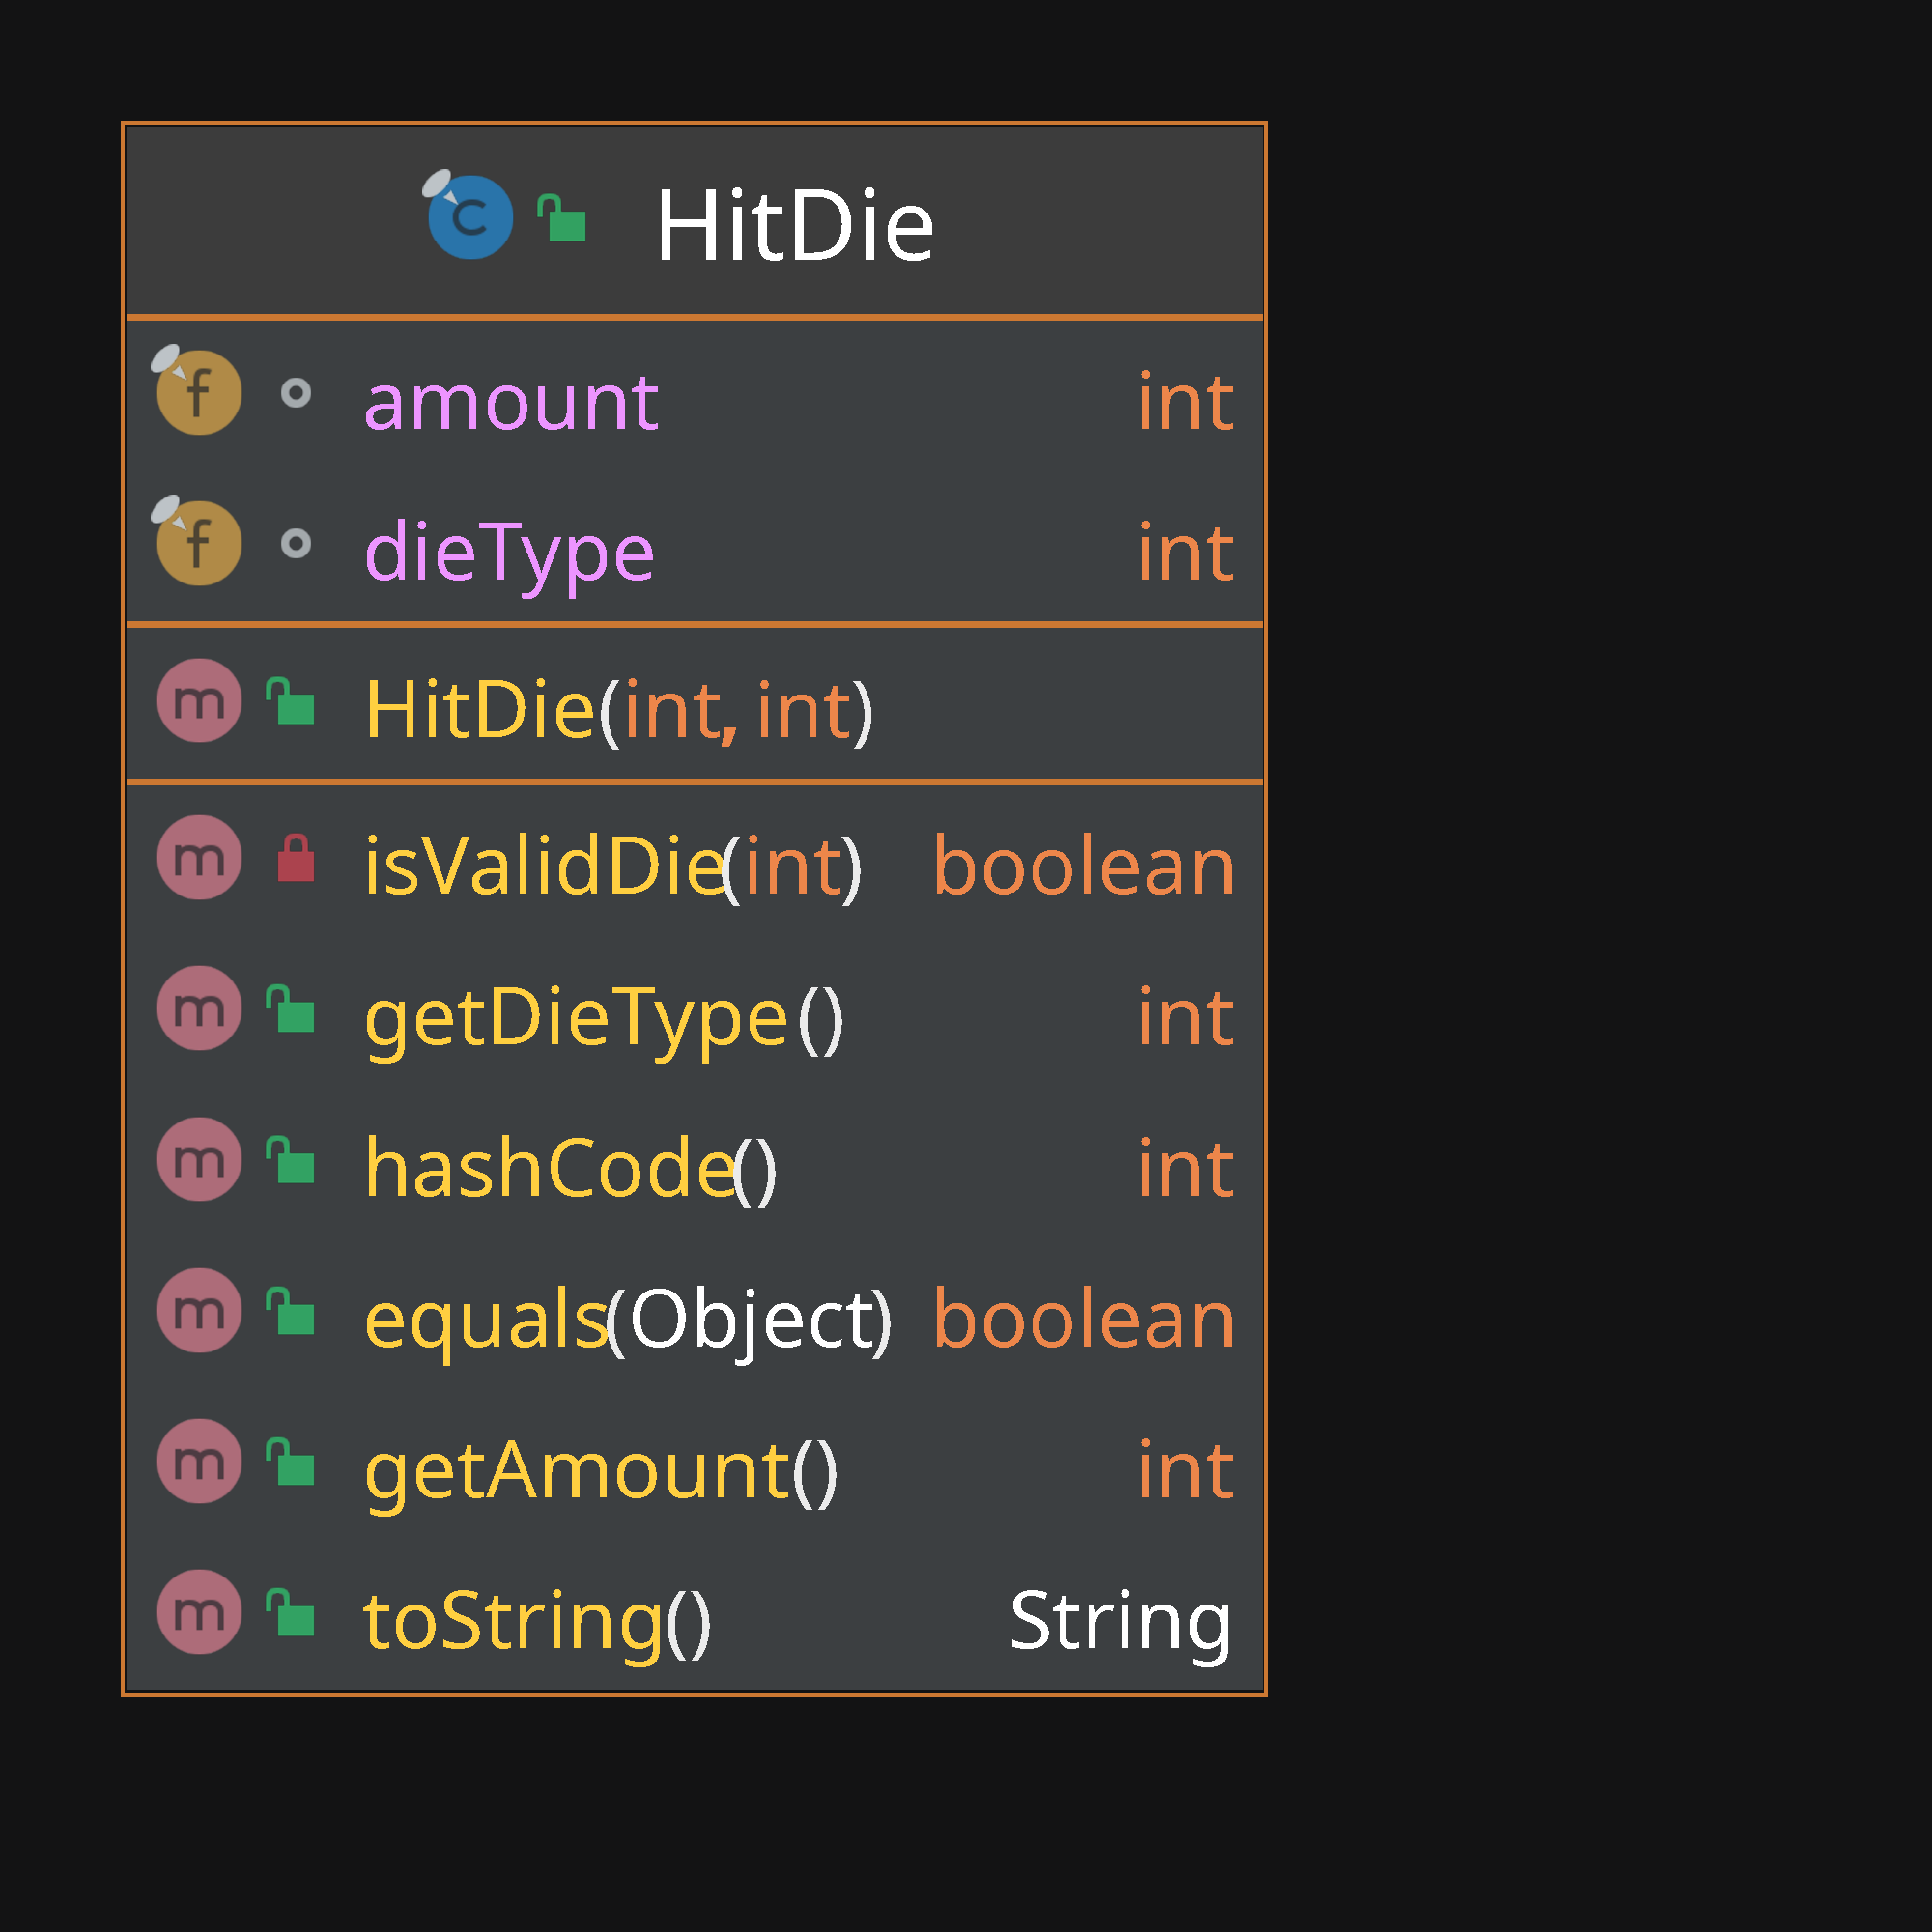
\includegraphics[width=0.4\textwidth]{Bilder/HitDie.pdf}
	\caption{UML der HitDie Klasse}
	\label{fig:HitDie-Solid}
\end{figure}
Abbildung \ref{fig:HitDie-Solid} zeigt das UML-Diagramm der \texttt{HitDie} Klasse. Sie hält das Single Responsibility Principle ein, da sie ausschließlich für die Repräsentation eines Würfels zuständig ist und keinerlei andere Funktionalität enthält.

\subsection{Negativ-Beispiel}
\begin{figure}[H]
	\centering
	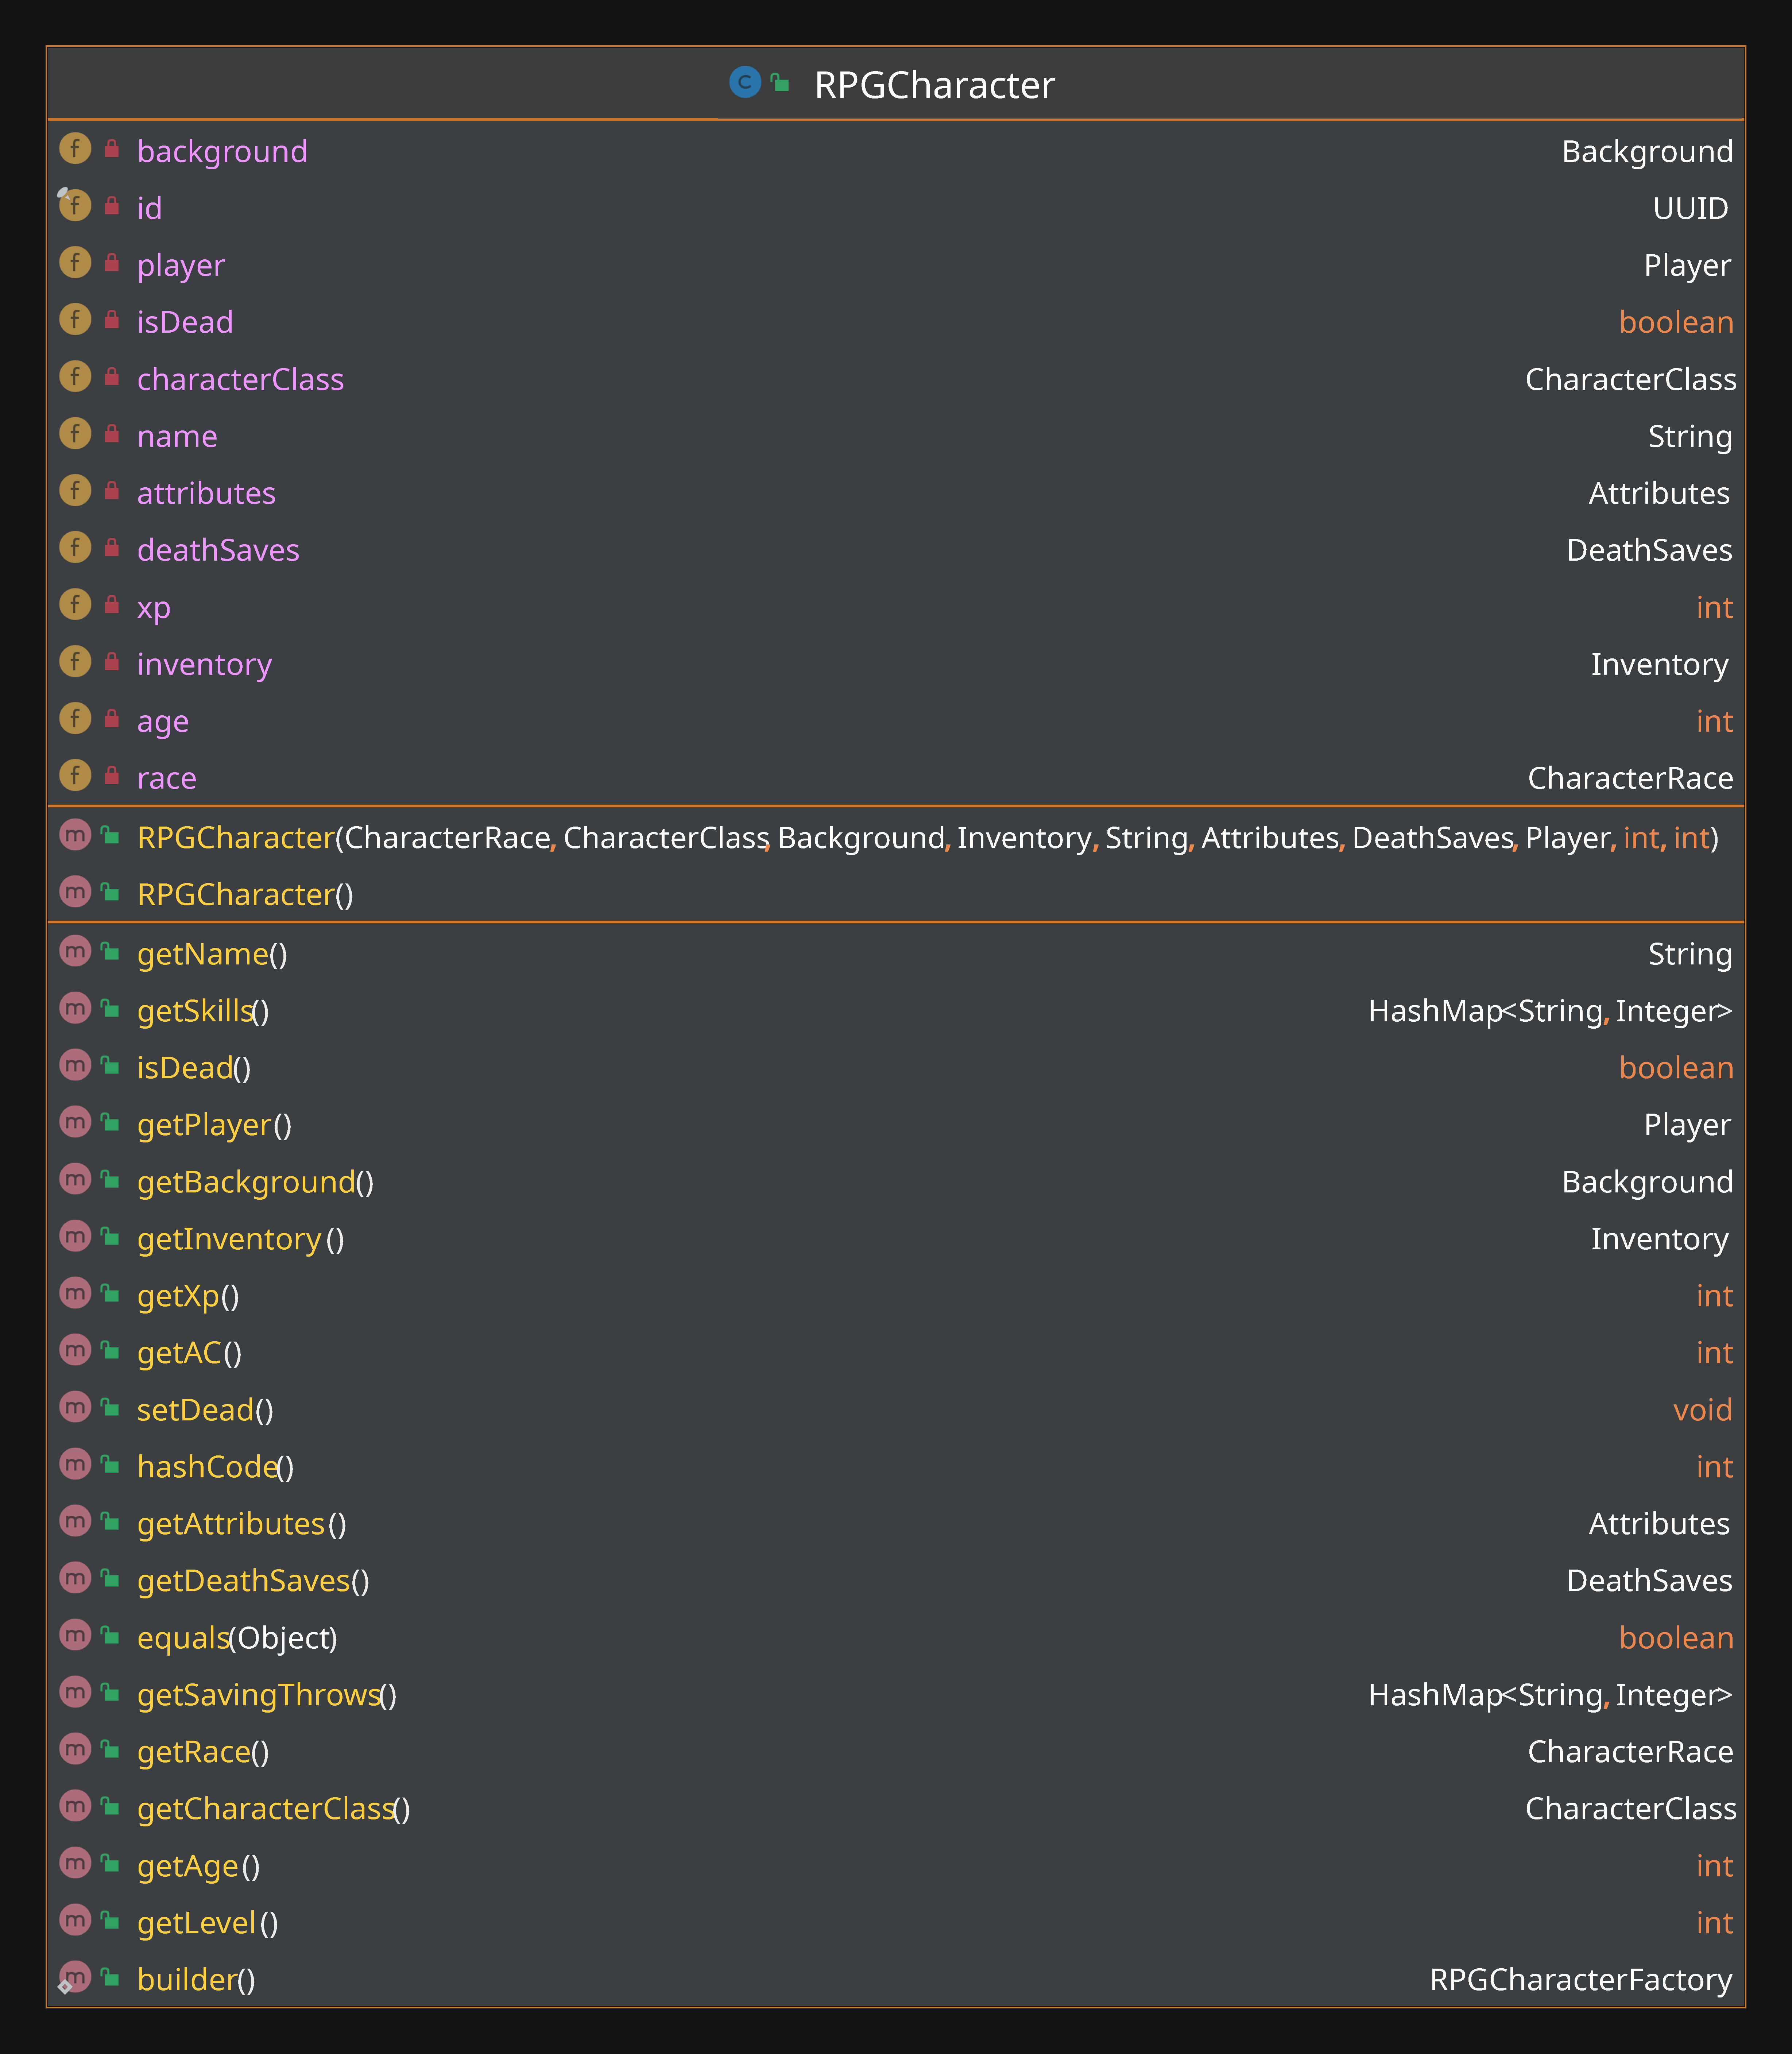
\includegraphics[width=0.4\textwidth]{Bilder/RPGCharacter.pdf}
	\caption{UML der RPGCharacter Klasse}
	\label{fig:RPG-Charadter}
\end{figure}
Die in Abbildung \ref{fig:RPG-Charadter} gezeigte \texttt{RPG-Character} Klasse hält das SRP nicht ein. Sie stellt nicht nur die verschiedenen Datenobjekte und Entitäten die ein Charakter hat zur Verfügung, sondern berechnet auch Status Werte wie z.B.: die ArmorClass (AC).  Daher wäre es sinnvoll diese Berechnung in eine eigene ArmorClass Klasse auszulagern, wie in Abbildung \ref{fig:RPG-CharadterSRP}.
\begin{figure}[H]
	\centering
	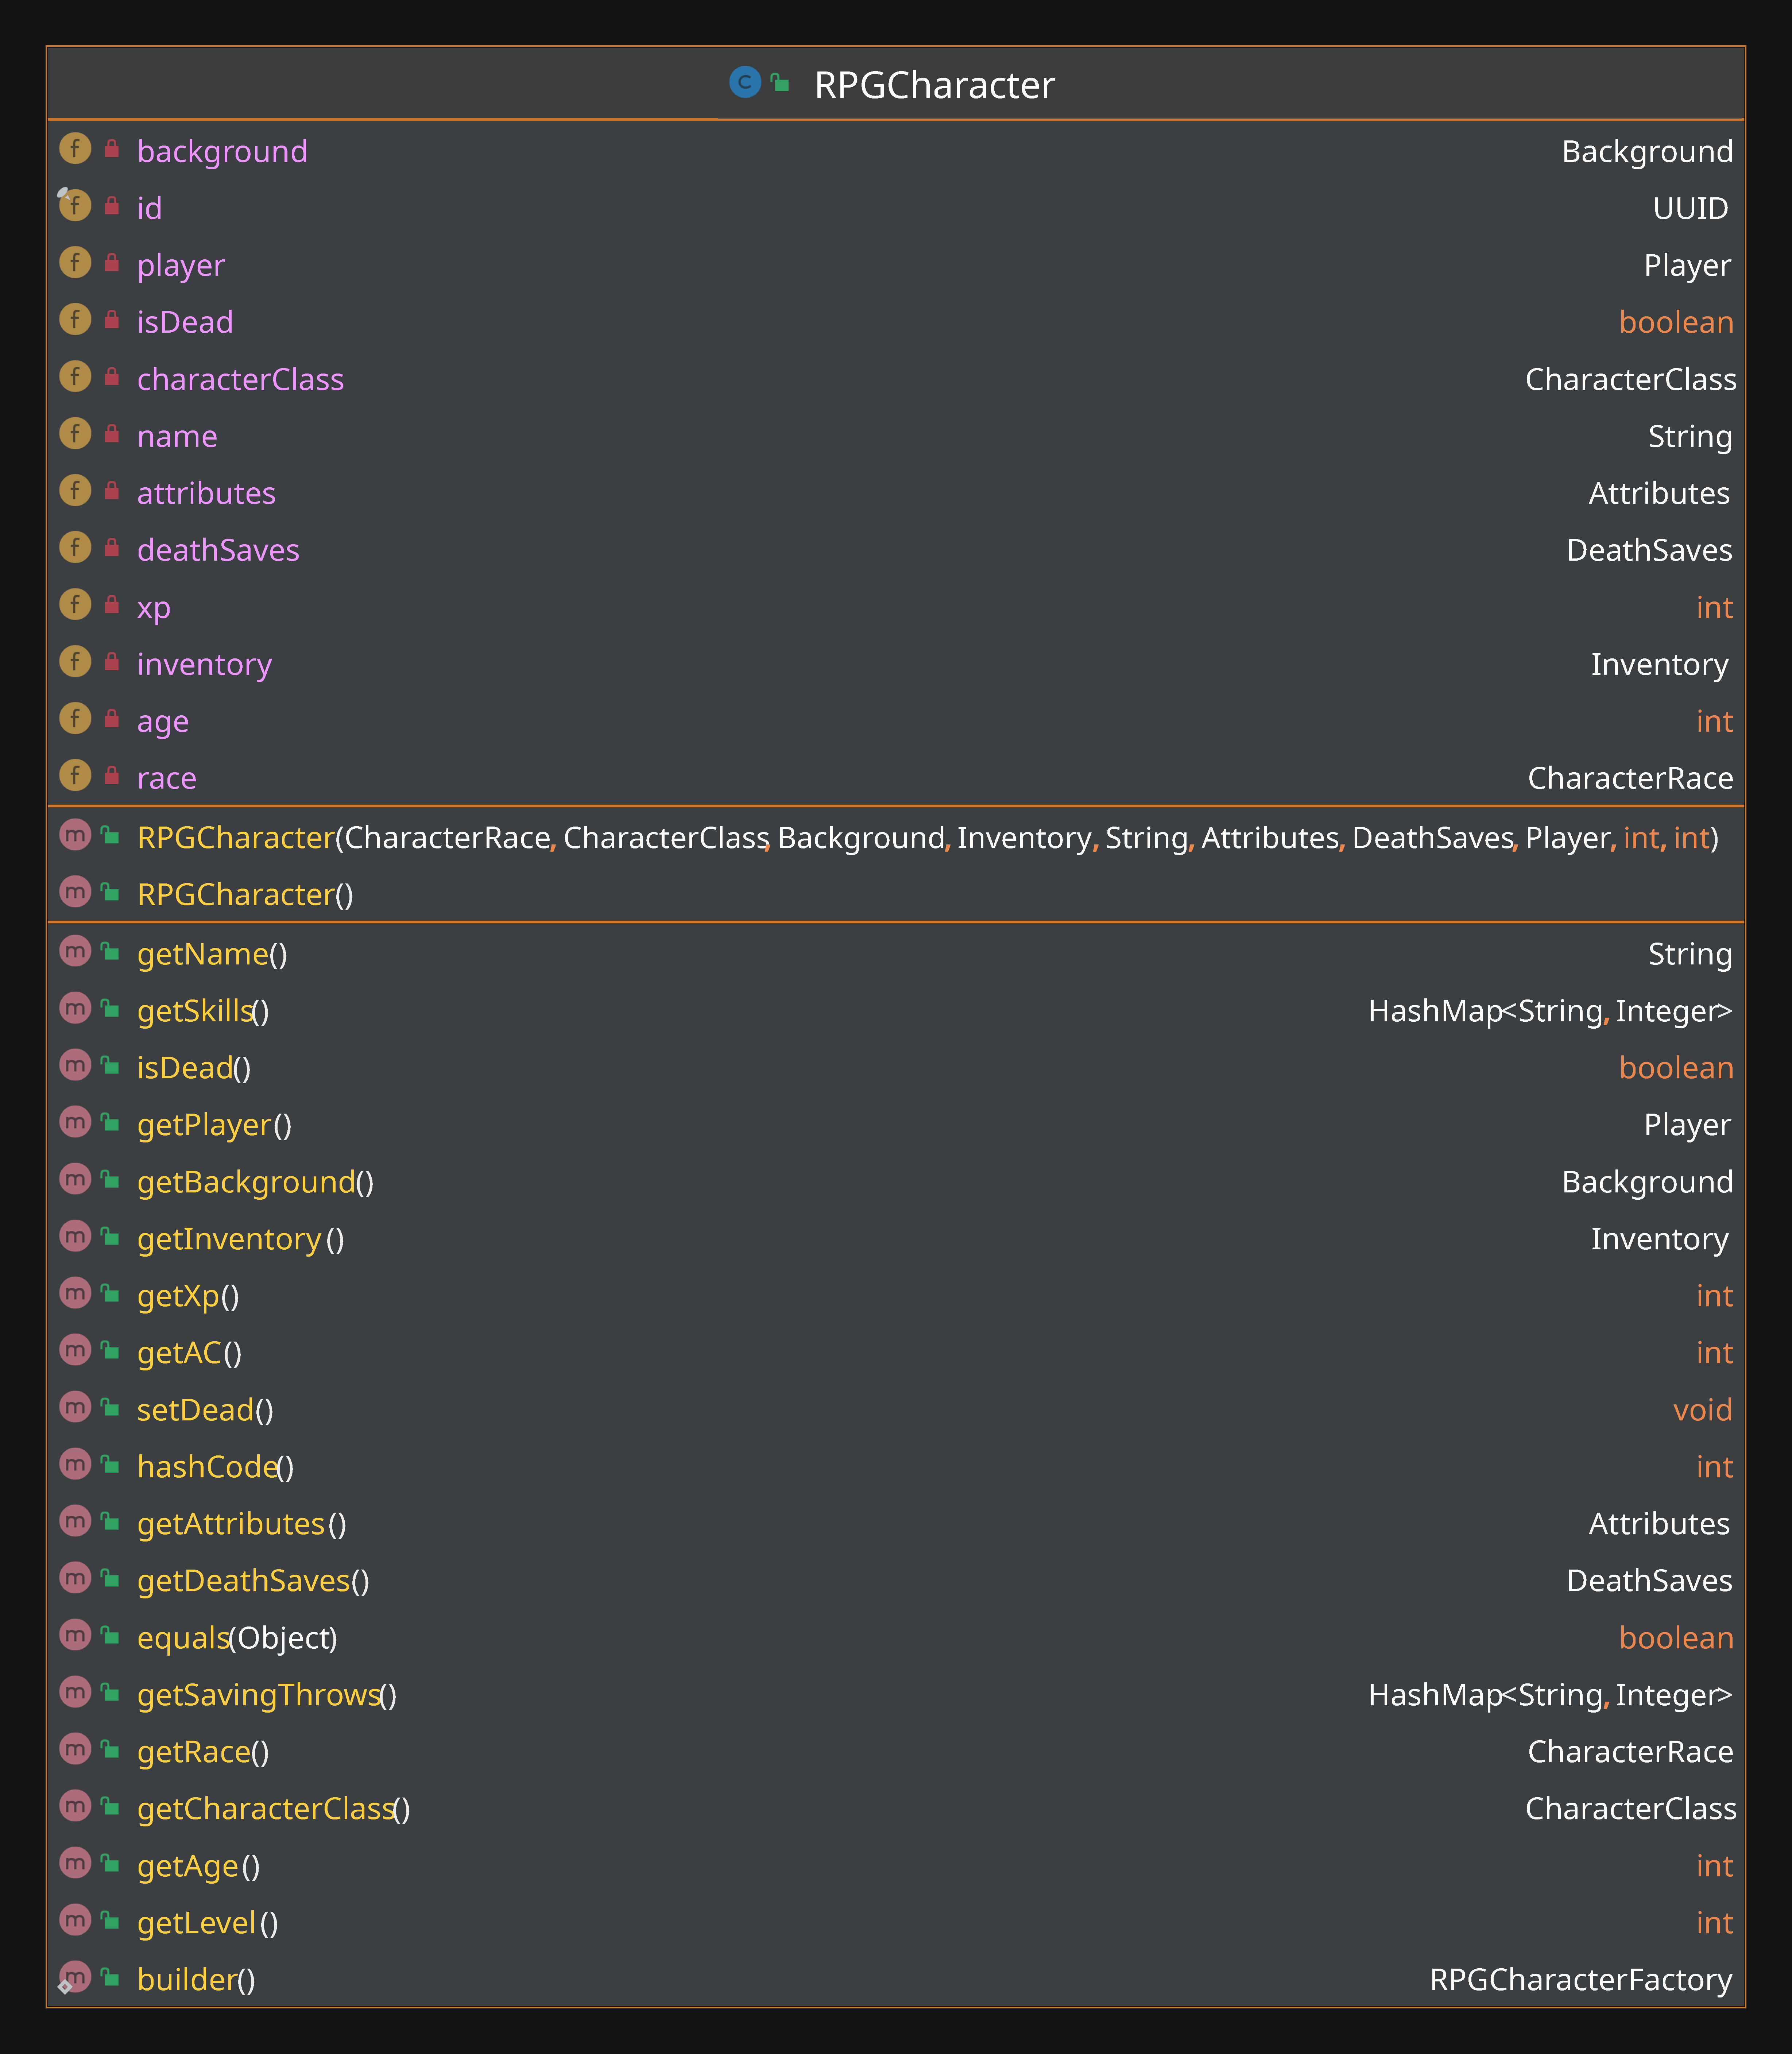
\includegraphics[width=0.4\textwidth]{Bilder/RPGCharacter.pdf}
		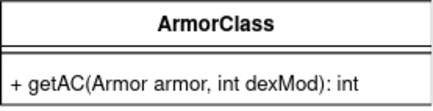
\includegraphics[width=0.4\textwidth]{Bilder/RPGCharacterSRP.drawio.pdf}
	\caption{UML der RPGCharacter Klasse und der theoretischen ArmorClass}
	\label{fig:RPG-CharadterSRP}
\end{figure}

\section{Analyse Open-Closed-Principle (OCP)}
\subsection{Positiv-Beispiel}
\begin{figure}[H]
	\centering
	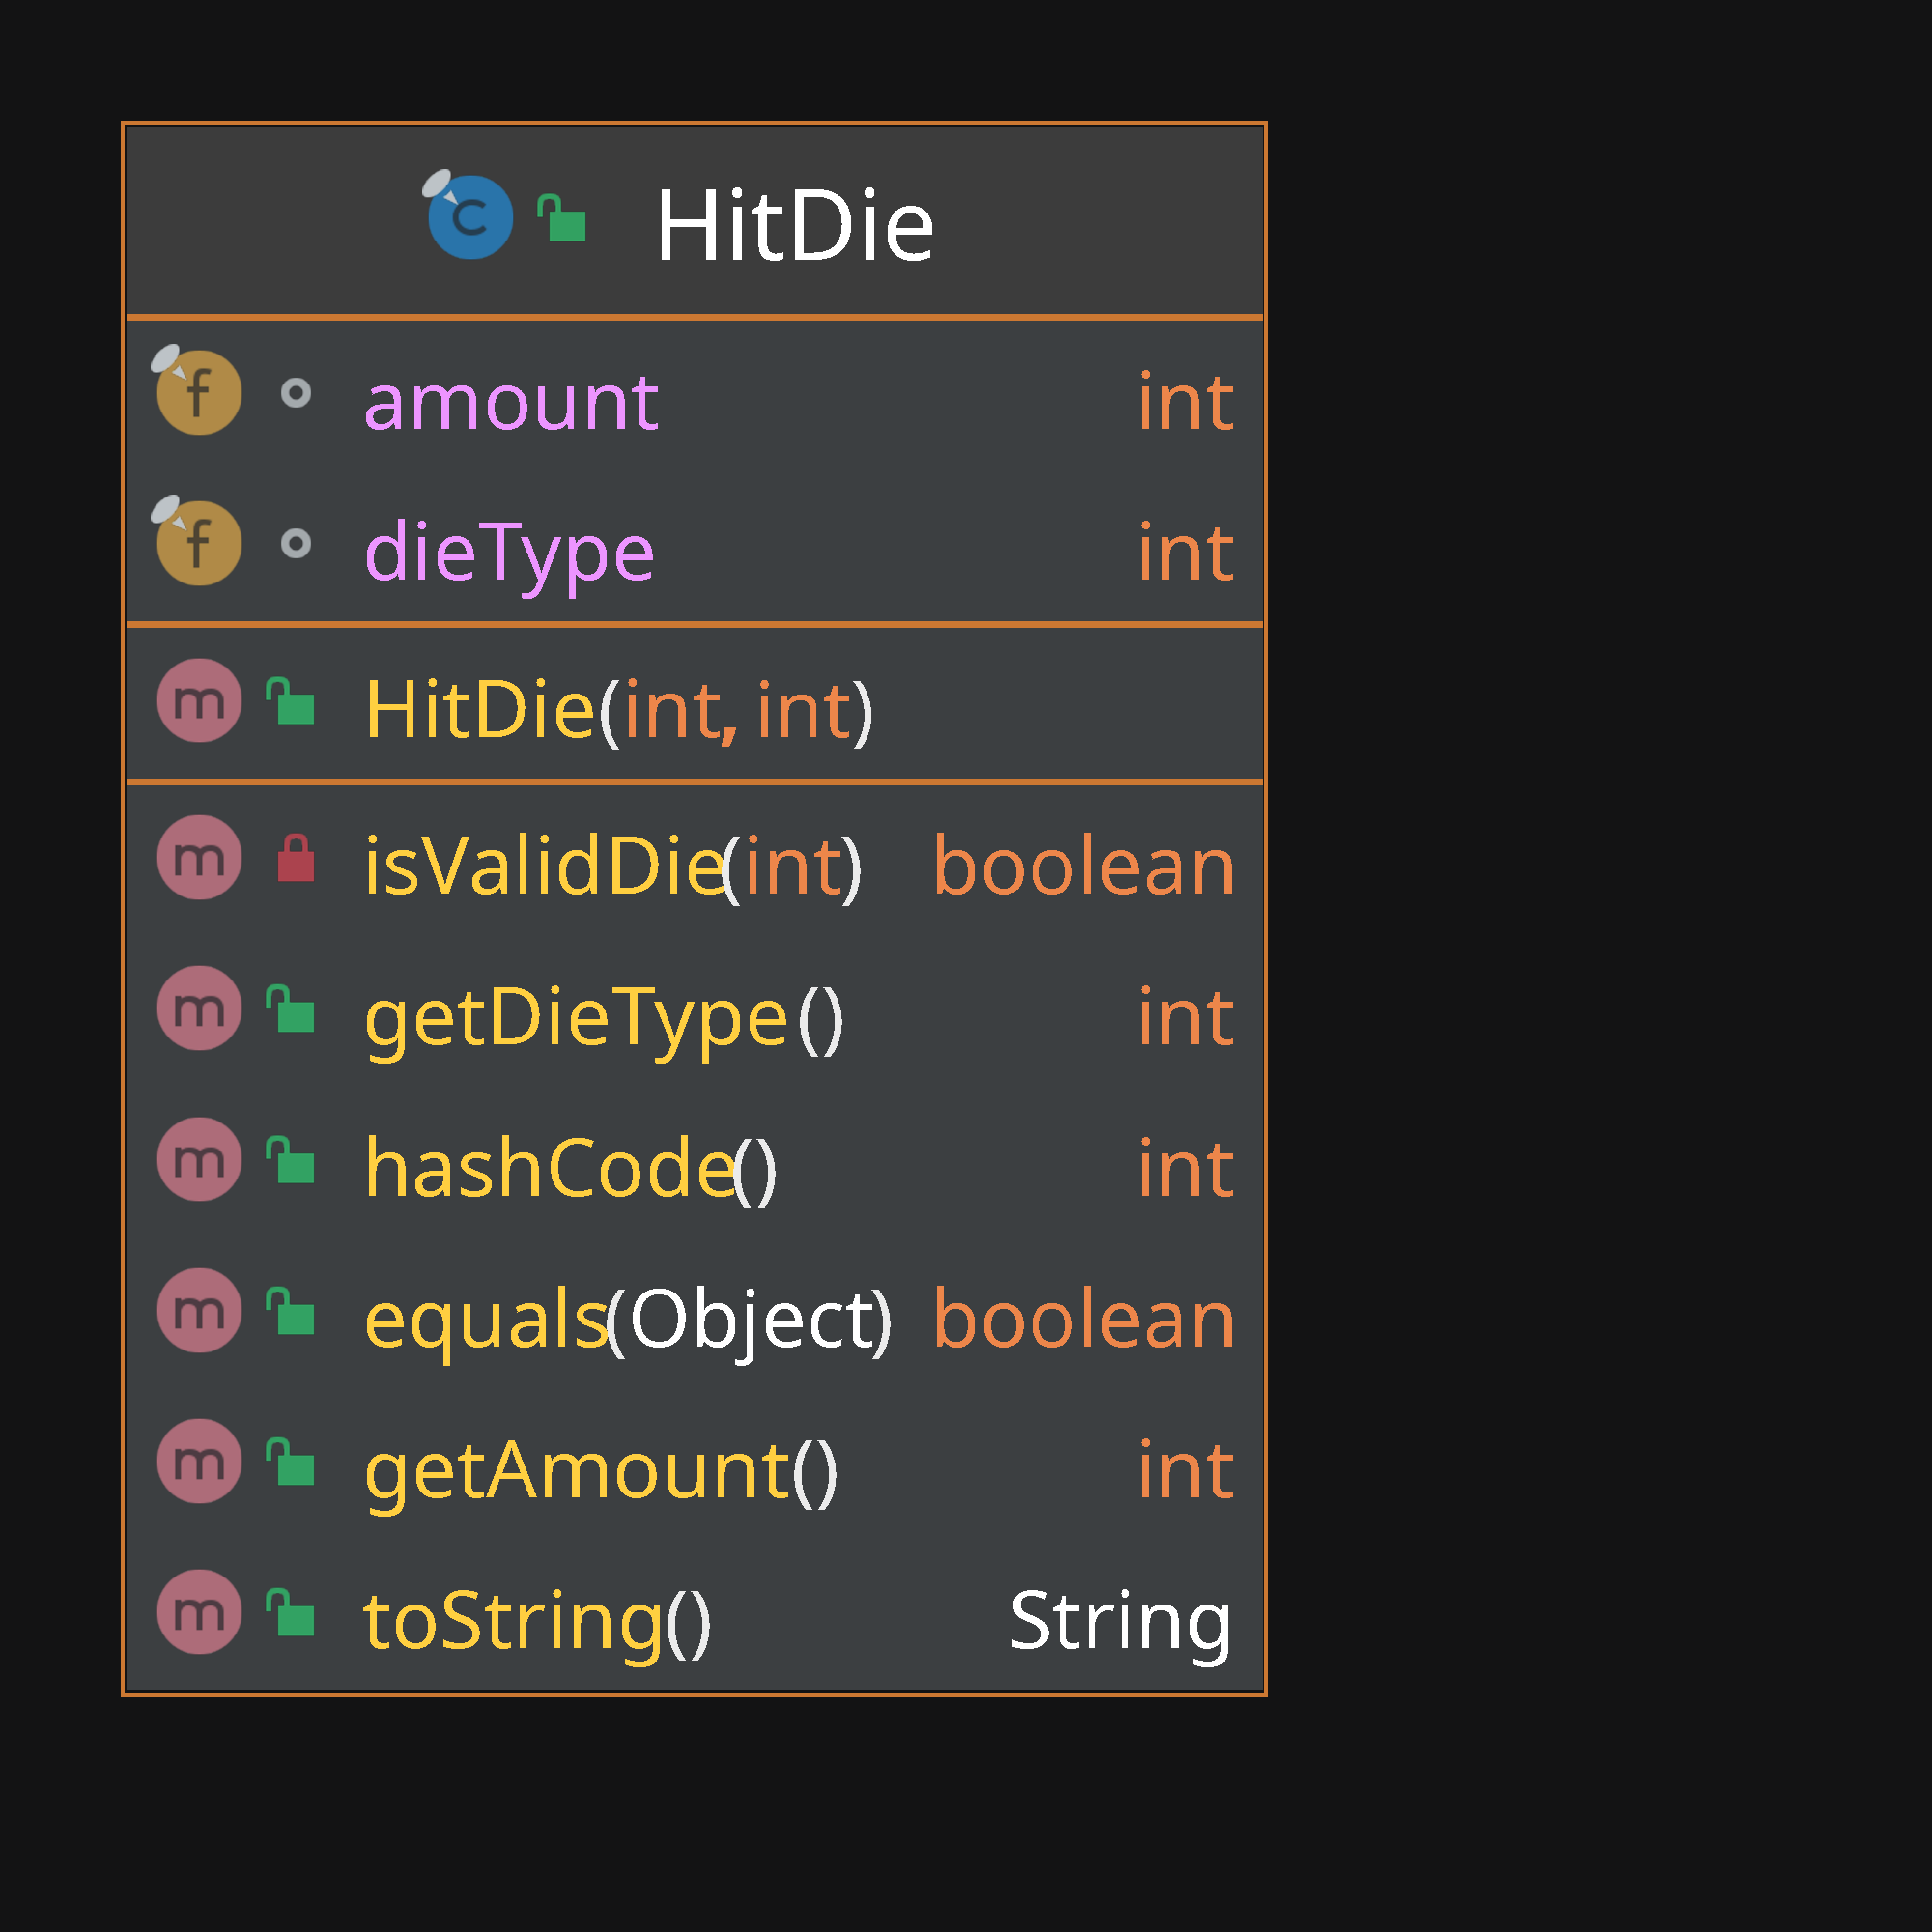
\includegraphics[width=0.4\textwidth]{Bilder/HitDie.pdf}
	\caption{UML der HitDie Klasse}
	\label{fig:HitDie-OCP}
\end{figure}
Die in Abbildung \ref{fig:HitDie-OCP} gezeigte Klasse \texttt{HitDie} hält das OCP ein, da sie alle Funktionen bereitstellt, die ein Würfel benötigt. Möchte man nun einen weiteren gültigen Würfel hinzufügen, muss nur diese Klasse angepasst werden und keine weiteren Änderungen im Projekt vorgenommen werden.
\subsection{Negativ-Beispiel}
Ich lasse an dieser Stelle das UML weg, da es keine Sinnvolle Aussagekraft hat. Die Klasse \texttt{SkillProficiencies} hält das OCP nicht ein, auch wenn sie eine Liste aller verfügbaren Skills enthält, muss man, wenn man einen neuen Skill hinzufügen möchte auch Änderungen in der \texttt{RPGCharacterClass} vornehmen. Da dort eine Hashmap zusammengebaut wird, die die tatsächlichen Werte enthalten. Somit liegt die Funktionalität der SkillProficiencies Klasse auf 2 Klassen aufgeteilt im Projekt und Änderungen und Modifikationen erfordern einen höheren Aufwand. Lösen könnte man dies, in dem man entweder in der Klasse SkillProficiencies eine neue Methode für die oben gennante Funktionalität anlegt, oder eine Klasse für die Skillwerte anlegt, die sich eine statische Liste aller validen Skills mit der SkillProficiencie Klasse teilt.

\section{Analyse Liskov-Substitution- (LSP), Interface-Segreggation- (ISP), Dependency-Inversion-Principle (DIP)}
\[jeweils eine Klasse als positives und negatives Beispiel für entweder LSP oder ISP oder DIP);  jeweils UML der Klasse und Begründung, warum man hier das Prinzip erfüllt/nicht erfüllt wird\] \\
\[Anm.: es darf nur ein Prinzip ausgewählt werden; es darf NICHT z.B. ein positives Beispiel für LSP und ein negatives Beispiel für ISP genommen werden\]
\subsection{Positiv-Beispiel}
\subsection{Negativ-Beispiel}
